

\actTitle{Worksheet 1.4}


\noindent \textbf{Instructions:}  Work together in groups of  3 or 4 to complete the following problems.




\begin{enumerate}
\item Let $f(x)$ be a linear function such that $\displaystyle f(2)=\frac{7}{3}$ and the graph of $f(x)$ is parallel to the line $2x+3y+4=0$. 
\begin{enumerate}
\item Determine $f(x)$ and write your final answer in \emph{slope-intercept} form. (Leave fractions in your answer, no decimals.)
\vfill
\item Graph $f(x)$ and  $2x+3y+4=0$ on the rectangular coordinate system below.\\
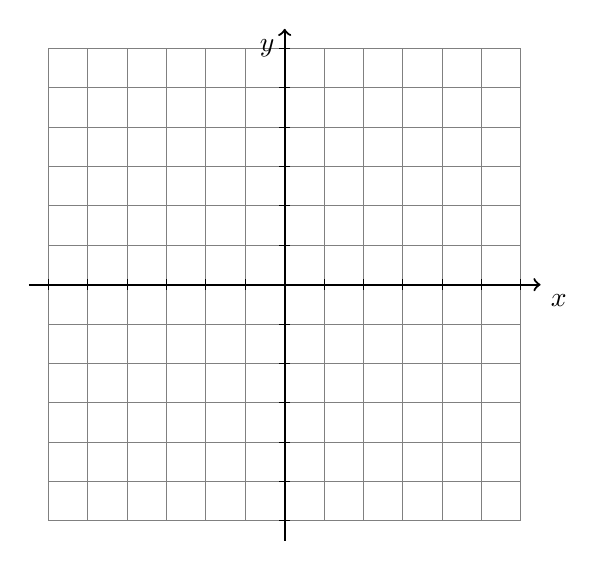
\begin{tikzpicture}[y=.5cm, x=0.5cm,font=\sffamily]
    %% ticks
    \draw[step = 1, gray] (-6,-6) grid (6,6);
    %% axis
    \draw[thick,->] (-6.5,0) -- coordinate (x axis mid) (6.5,0) node[anchor = north west] {$x$};
    \draw[thick,->] (0,-6.5) -- coordinate (y axis mid) (0,6.5) node[anchor = north east] {$y$};
    \foreach \y in {-6,-5,...,-1,1,2,...,6} {
      \draw (2pt, \y) -- (-2pt, \y);
    }
    \foreach \x in {-6,-5,...,-1,1,2,...,6} {
      \draw (\x,2pt) -- (\x,-2pt);
    }

  \end{tikzpicture}

\item Determine the domain and range of $f(x)$.\\[.5in]
\end{enumerate}


\newpage
\item Determine whether the lines $y= 2x+3$ and and $x-3y-5=0$ are parallel, perpendicular, or neither. \vfill


\item Determine an equation of the \emph{vertical} line which passes through the point $(-2, 3)$. Then determine an equation of the \emph{horizontal} line through $(-2,3)$.\vfill

\newpage

\item Consider the function $f(x)=x^2-3x+2$.
\begin{enumerate}
\item Algebraically determine the average rate of change of $f(x)=x^2-3x+2$ between $x_1=1$ and $x_2=3$.
\vfill



\item The graph of $f(x)=x^2-3x+2$ is given below.  Draw a line between the points $(1,f(1))$ and $(3,f(3))$.\\

%\begin{tikzpicture}[scale=1]
%	\begin{axis}[
%	                   axis equal,
%	                   axis line style = thick,
%	                   axis x line=middle, 
%	                   axis y line=center, 
%	                   minor tick num = 3,
%	                   grid = both,
%	                   major grid style={black!70},
%	                   minor grid style ={gray!70},
%	                   xtick={-4,-2,0,2,4,6},
%	                   ytick={-2,0,2,4,6,8},
%	                   xmin = -4,
%	                   xmax = 6,
%	                   ymin = -2.25,
%	                   ymax = 8.25,
%	                   tick align=outside,
%	                   style={font=\tiny}]
%
%		\addplot+[mark=none,smooth, style={thick}] (\x,{\x*\x-3*\x+2});
%		\addplot[only marks, style={mark size=1pt}] table {
%		0 2
%		1 0
%		1.5 -.25 
%		2 0
%		};
%	\end{axis}
%\end{tikzpicture}

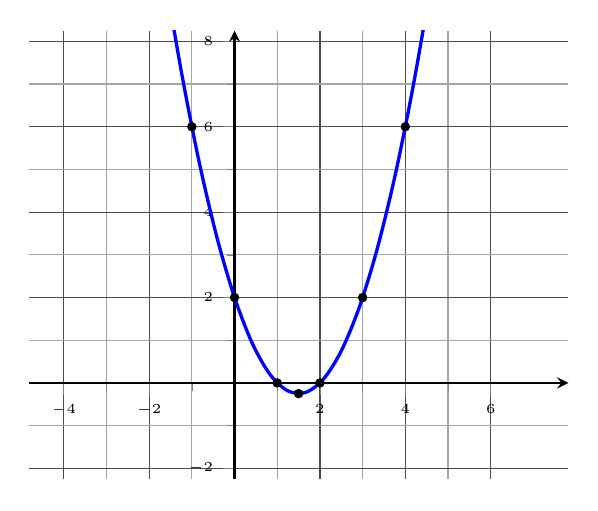
\begin{tikzpicture}[scale=1]
	\begin{axis}[
	                   axis equal,
	                   axis line style = thick,
	                   axis x line=middle, 
	                   axis y line=center, 
	                   minor tick num = 1,
	                   grid = both,
	                   major grid style={black!70},
	                   minor grid style ={gray!70},
	                   xtick={-4,-2,0,2,4,6},
	                   ytick={-2,0,2,4,6,8},
	                   xmin = -3,
	                   xmax = 6,
	                   ymin = -2.25,
	                   ymax = 8.25,
	                   tick align=outside,
	                   style={font=\tiny}]

		\addplot+[mark=none,smooth, style={very thick}] (\x,{\x*\x-3*\x+2});
		\addplot[only marks, style={mark size=1.5pt}] table {
		0 2
		1 0
		1.5 -.25 
		2 0
		3 2
		4 6
		-1 6
		};
	\end{axis}
\end{tikzpicture}

\item Find the slope of the line between the points $(1,f(1))$ and $(3,f(3))$ on $f(x)=x^2-3x+2$.
\vfill
\item What do you notice about the slope of the line between the points $(1,f(1))$ and $(3,f(3))$ on $f(x)=x^2-3x+2$ and the average rate of change of $f(x)=x^2-3x+2$ between $x_1=1$ and $x_2=3$.\\[.5in]
\end{enumerate}

\newpage

\item Consider the line $x+2y=3$.
\begin{enumerate}
\item Find the $x$ and $y$ intercepts of the line.
\vfill
\item Determine the distance between the $x$-intercept and the $y$-intercept.
\vfill 
\item Find the slope of the line $x+2y=3$.
\vfill
\end{enumerate}

\end{enumerate}
















